\begin{boxK}
    \lr{
        \lstinputlisting[language = Python]{Final/code/twoFish/encrypt.py}
    }
\end{boxK}


\begin{boxK}
    \lr{
        \lstinputlisting[language = Python]{Final/code/twoFish/decrypt.py}
    }
\end{boxK}

\begin{boxB}
    این کد پایتون یک پیاده سازی از الگوریتم رمزنگاری دو ماهی است. دو ماهی یک رمز بلوکی متقارن است که فقط 16 بایت را در هر بار رمزنگاری می کند. این کد از پیاده سازی C بهینه شده بروس شنایر (https://www.schneier.com/code/twofish-optimized-c.zip) استفاده می کند. این کد شامل توابع زیر است:

 \lr{to32Char(X):}
 
این تابع یک عدد 32 بیتی را به چهار بایت تبدیل می کند.
 
 \lr{bytesTo32Bits(l):} 
 
 این تابع یک لیست از بایت ها را به یک عدد 32 بیتی تبدیل می کند.

 \lr{ROR(x, n) , ROL(x, n):}
 
 این توابع عملگرهای شیفت راست و چپ روی بایت ها را پیاده سازی می کنند.
 
 \lr{ROR4(x, n):} 
 
این تابع عملگر شیفت راست روی 4 بیت را پیاده سازی می کند.

 \lr{polyMult(a, b)  , gfMult(a, b, modulus):}
 
 این توابع ضرب دو عدد در حلقه های گالوآ را پیاده
 سازی می کنند.

\lr{gfMod(t, modulus):} 

این تابع باقی مانده یک عدد در حلقه گالوآ را پیدا می کند.

\lr{matrixMultiply(md, sd, modulus):}

این تابع ضرب دو ماتریس در حلقه گالوآ را پیدا می کند.

\lr{printRoundKeys(K): }

این تابع کلیدهای دور رمزنگاری را نمایش می دهد.

\lr{keySched(M, N):}

این تابع برنامه کلید رمزنگاری را از چکیده کلید M با طول N بایت تولید می کند.

\lr{makeKey(Me, Mo, k):} 

این تابع کلیدهای دور رمزنگاری را با استفاده از تابع h و ضرب MDS تولید می کند.

\lr{h(X, L, k):}

این تابع چکیده X با استفاده از لغات L و جدول های Q0 و Q1 را پیدا می کند.

بخش دوم کد را دریافت کردم. این کد شامل توابع زیر است:

\lr{Qpermute(x, Q):}

این تابع یک عدد 4 بیتی را با استفاده از جدول Q معکوس می کند.

\lr{F(R0, R1, r, K, k, S):}

این تابع تابع F در الگوریتم دو ماهی را پیاده سازی می کند. این تابع دو عدد 32 بیتی R0 و R1 را گرفته و با استفاده از تابع g و کلیدهای دور K، دو عدد 32 بیتی F0 و F1 را برمی گرداند.

\lr{encrypt(K, k, S, PT):}

این تابع یک بلوک 16 بایتی PT را با استفاده از کلید K، طول کلید k و لغات S رمزنگاری می کند. این تابع شامل سه مرحله است: سفید کردن ورودی، دور های رمزنگاری و سفید کردن خروجی.

\lr{decrypt(K, k, S, PT):}

این تابع یک بلوک 16 بایتی PT را با استفاده از کلید K، طول کلید k و لغات S رمزگشایی می کند. این تابع شامل سه مرحله است: سفید کردن ورودی، دور های رمزگشایی و سفید کردن خروجی.
\end{boxB}


\begin{boxB}
    
\lr{testKey(K, k, S):}

این تابع یک آزمون ساده برای الگوریتم دو ماهی را اجرا می کند. این تابع یک بلوک صفر را با استفاده از کلید K، طول کلید k و لغات S رمزنگاری و رمزگشایی می کند و نتایج را نمایش می دهد.

\lr{dispLongList(v):}

این تابع یک لیست از اعداد 32 بیتی را به صورت 16 رقم هگزادسیمال نمایش می دهد.



\lr{Itest128() , Itest192() , Itest256():}

این توابع آزمون های مختلف برای الگوریتم دو ماهی با طول های کلید مختلف را اجرا می کنند. این توابع هر بار چکیده خروجی قبل را به عنوان کلید جدید استفاده می کنند.

\lr{bench():}

این تابع زمان لازم برای رمزنگاری و تولید کلید با الگوریتم دو ماهی را سنجش می کند.


تمامی کدهای بالا در فایل 
main.py
موجود است.

فلوچارت کلی الگوریتم در تصویر زیر مشهود است.
\end{boxB}

\begin{figure}[h]
    \centering
    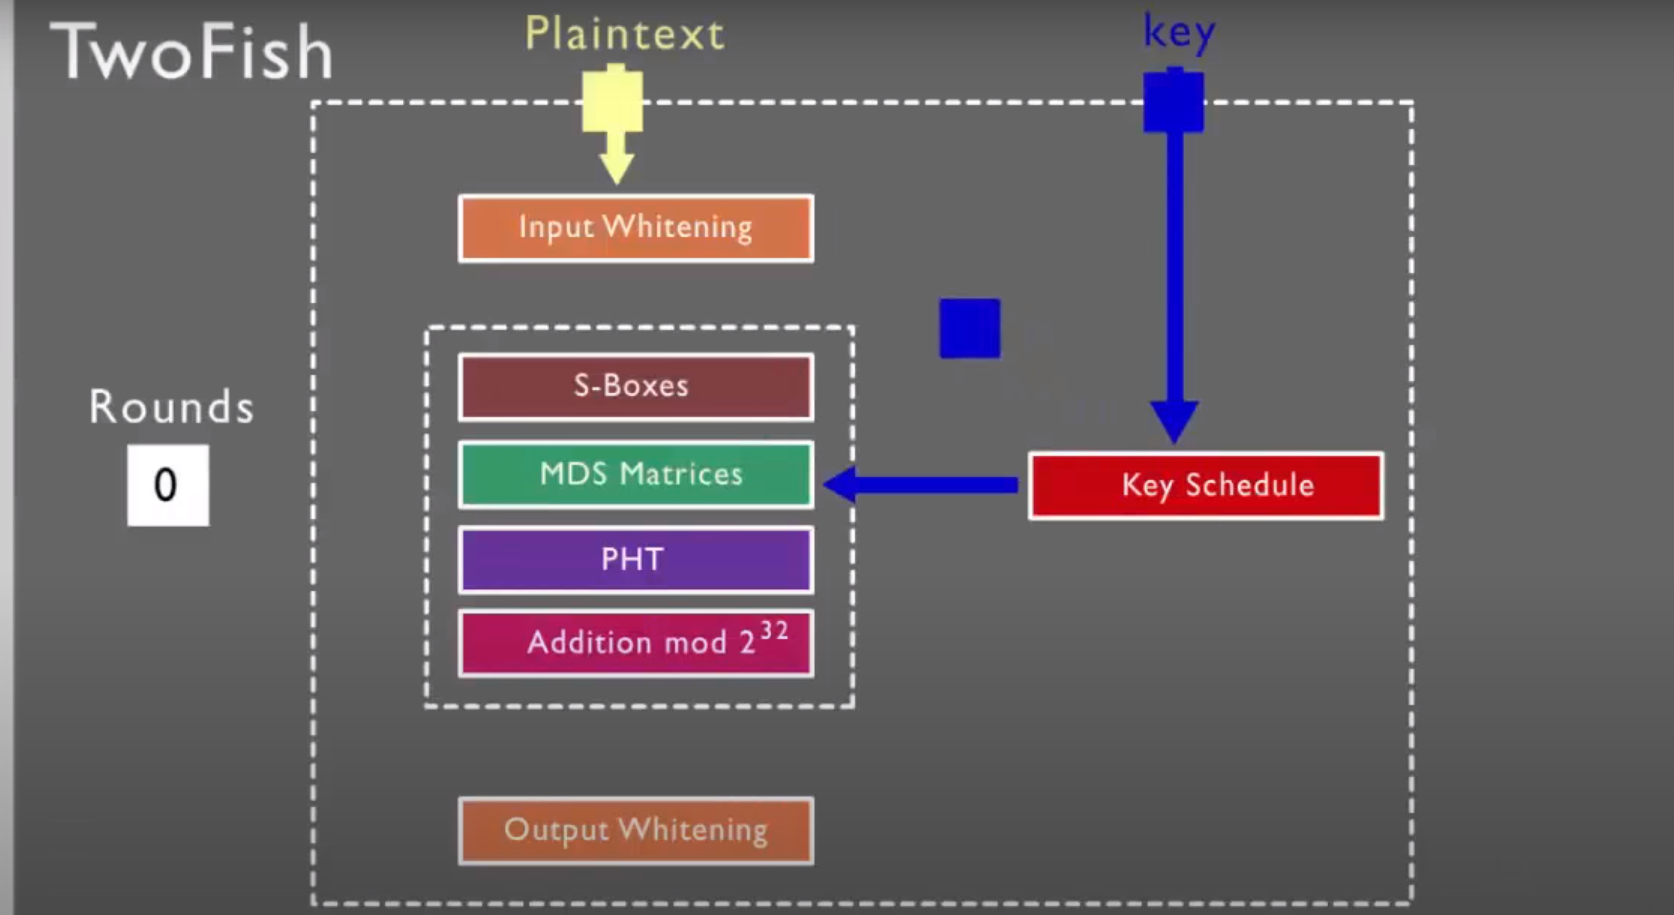
\includegraphics
    [width = 0.8\textwidth]
    {Final/images/twoFish.png}
    \caption{\lr{twoFish Algorithm}}
    \label{fig:enter-label}
\end{figure}